\section{Collaborative ML Workload Optimizations} \label{sec-ml-workloads}
In this section, we discuss the details of the Experiment Graph construction and workflow of our system and optimization process.
Next, we show how a real collaborative data science platform can benefit from our system through an example.

\subsection{Experiment Graph Representation}\label{sub-graph-construction}
\textbf{Workload DAG.}
A machine learning workload can be represented using a directed acyclic graph (DAG).
In the DAG, vertices represent the artifacts, i.e., raw or preprocessed data (represented by data frame objects) and machine learning models resulting from feature engineering and model training operations and edges represent the operations in the workload.
Each workload DAG has one or more initial vertices representing the raw datasets which are defined as part of the task definition in a collaborative platform.
We refer to the initial vertices as the roots.

\textbf{Experiment Graph. }
For every task, the collection of all the DAGs of the previously executed machine learning workloads forms a rooted graph (with potentially multiple root vertices) which we refer to as the \textit{experiment graph}.
More formally, we represent the experiment graph by $G(V, E)$.
$V=\{v_i\}, i = 1, \cdots, n$ is the set of all the artifacts in all the workload DAGs.
$E=\{e_i\}, i = 1, \cdots, m$ is the set of all the executed operations in the workload DAGs.
A directed edge $e$ from $v_i$ to $v_j$ in $G(V, E)$ indicates that the artifact $v_j$ is derived from the artifact $v_i$ by applying the operation in $e$.
Every vertex $v$ has the attributes $\langle f, s \rangle$ (accessed by $v.f$ and $v.s$) which represent the frequency, i.e., number of different workloads an artifact appeared in, and storage size of the artifact.
Every edge $e$ has the attribute $\langle t \rangle$ (accessed by $e.t$) which represents the run-time (in seconds) of the operation.

Inside each vertex, we store the meta-data of the artifact.
Depending on how \textit{useful} an artifact is, we may also store the actual underlying data inside the artifact (Section \ref{sec-materialization}).
If the artifact is a raw or a preprocessed dataset, then its meta-data includes the name, type, and total size of each column of the data and its underlying data is represented by the dataframe object (i.e., Pandas dataframe). 
If the artifact is a machine learning model, its meta-data includes the name, type, hyperparameters, and the error metric of the model and its underlying data is consist of the model weights.
Each edge contains the meta-data of the operation it represents, such as the function name, training algorithm, and hyperparameters.
To uniquely identify an edge, we utilize a hash function which receives as input the operation and its hyperparameters (if it has any).
Since the experiment graph is rooted, we assign a hash value to every vertex which is computed in the following way:
\[
    h(v)= 
\begin{cases}
    id,& \text{if } v \text{ is root}\\
    h\Big(\sum\limits_{e \in in\_edge(v)} (h(e.source) + h(e) ) \Big)  ,              & \text{otherwise}.
\end{cases}
\]
where $in\_edge(v)$ returns the edges with destination $v$. 
Intuitively, the hash of a root vertex is its unique identifier (location on disk or download URL) and the hashes of other vertices are derived recursively by combining the hashes of their parents and edges which connect them to their parents.
%This hashing procedure results in two important properties.
%
%\textit{Property 1}.
%The two vertices, $v_1$ and $v_2$ in graphs $G_1$ and $G_2$ are the same if and only if $h(v_1)$ in $G_1$ is the same as $h(v_2)$ in $G_2$.
%
%\textit{Property 2}.
%If a vertex $v_1$ in graph $G_1$ does not exist in $G_2$ , then no successors of $v_1$ can exist in $G_2$.}

After a machine learning workload is executed, we update the experiment graph by adding the new artifacts and operations.
If any of the artifacts already exist in the graph, their frequency is updated.

\textbf{Workload DAG generation.}
Instead of designing a new DSL, we extend the existing Pandas and scikit-learn \cite{sklearn_api} python packages which are frequently used for data analysis and machine learning workloads.
Listing \ref{listing-experiment-graph} shows an example of a workload script.
With only a slight modification of the import commands, we are able to load our system's modules.
A parser component reads the user code and instead of executing it line-by-line, it creates the edges and vertices of the workload DAG.
The actual execution is invoked with \textit{.get()} command of a vertex (Line 18, Listing \ref{listing-experiment-graph}.
Figure \ref{fig-experiment-graph}a shows an example graph constructed from the code in Listing  Listing \ref{listing-experiment-graph}.
\begin{figure}
\begin{subfigure}[b]{0.4\linewidth}
\centering
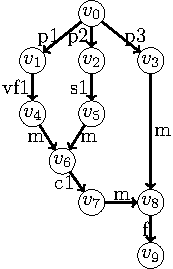
\includegraphics[width=0.8\linewidth]{../images/tikz-standalone/example-graph}
\caption{}
\end{subfigure}%
\begin{subfigure}[b]{0.6\linewidth}
\begin{tabular}{lcl}
\hline
operation & label &  hash \\
\hline
project(ad..) & $\langle 2s\rangle$ &p1 \\
project(ts, ..) & $\langle 6s\rangle$ & p2\\
project(y) & $\langle 2s\rangle$ & p3\\
vectorizer.f\_t & $\langle 40s\rangle$ & vf1 \\
selector.f\_t & $\langle 60s\rangle$ & s1 \\
concat & $\langle 10s\rangle$ & c1 \\
merge & $\langle 0s\rangle$ & m\\
svm.fit & $\langle 100s\rangle$ & f\\
\hline
\end{tabular}
\caption{}
\end{subfigure}
\caption{Experiment graph constructed from the Listing \ref{listing-experiment-graph} (a) and the hash of the operations in the scripts (b)}
\label{fig-experiment-graph}
\end{figure}
Table \ref{fig-experiment-graph}b shows both the label of every edge operation, i.e., time, and the hash of the operations and their hyperparameters.

\begin{lstlisting}[language=Python, caption=Example script,captionpos=b,label = {listing-experiment-graph}]
import custom_pandas as pd

from custom_sklearn import svm
from custom_sklearn.feature_selection import SelectKBest
from custom_sklearn.feature_extraction.text import CountVectorizer

train = pd.read_csv('../input/train.csv') 
print train.columns # [ad_desc,ts,u_id,price,y]
vectorizer = CountVectorizer()
count_vectorized = vectorizer.fit_transform(train['ad_desc'])
selector =  SelectKBest(k=2)
top_features = selector.fit_transform(
                                  train[['ts','u_id','price']],  
                                  train['y'])
top_features # print the content of the data frame			     
X = pd.concat([count_vectorized,top_features], axis = 1)
model = svm.SVC().fit(X, train['y'])
model.get()
\end{lstlisting}

We start with an empty Experiment Graph.
After the execution of the script and updating the Experiment Graph, all the artifacts (vertices) have a frequency of 1.
In order to represent operations which process multiple input artifacts, e.g., concat and svm.fit operations in Listing \ref{listing-experiment-graph}, we proceed as follows.
First, we merge the vertices representing the artifacts into a single vertex using a merge operator.
The merge operator is a logical operator which does not incur a cost, i.e., it has a run-time of 0 seconds.
The merged vertex is also a logical vertex with no actual attributes which only contains the vertex ids of the merged vertices.
Then, we draw an edge from the merged vertex which represents the actual operation.
For example, in Figure \ref{fig-experiment-graph}a, before applying the concatenation operation, we merge $v_4$ and $v_5$ into $v_6$, then we apply the concatenation operation (c1).
Furthermore, when computing the hash of a merged vertex, we take the merge order into account.
For example, the operation svm.fit has $X$ (represented by $v_7$) as first argument and train['y'] (represented by $v_3$) as its second argument.
When computing hash of $v_8$, we combine the parents in the same order, i.e., $h(v_8) = h(h(v_7) + m + h(v_3) + m)$. 
After the DAG is constructed, its execution is invoked with the call to the $get()$ command on Line 18.

\subsection{System Architecture and Workflow}
Figure \ref{system-workflow} shows the components of the collaborative workload optimizer system.
First, a parser component generates the workload DAG from the user scripts (Step 1).
Upon the invocation of the $get()$ method of an artifact, a local optimization process beings.
The local optimizer extracts the subgraph which must be executed in order to compute the terminal vertex.
The local optimizer traverses the graph in reverse order starting at the terminal vertex until the root vertices.
It stops the traversal when it reaches a previously computed vertex.
In interactive workloads, it is likely that many of the intermediate vertices between the terminal vertex and the root vertices are previously computed.
The subgraph of all the visited vertices and the edges connecting them is another DAG, which we refer to as the \textit{local execution DAG}, and is the result of the local optimizer (Step 2).
%For example in Figure \ref{system-workflow}, the traversal begins at Vertex 7 and continues until it visits Vertices 2 and 3.
%Since both Vertices are already computed (depicted with black color), the traversal stops and returns the subgraph starting at Vertices 2 and 3. 
The global optimizer component receives the local execution DAG and looks for optimization opportunities, i.e., reusing materialized vertices or warmstarting model training, in the experiment graph.
The result of the global optimization process is another subgraph, which we refer to as the \textit{global execution DAG} (Step 3).
%For example, in Figure \ref{system-workflow}, the experiment graph has previously materialized the underlying data (Dataset, Aggregate, or Model) of Vertex 5.
%Therefore, during the global optimization, the underlying data of Vertex 5 is transferred to the workload which results in another subgraph with Vertex 3 and Edge $e_4$ pruned.
Then, an execution planner receives the global execution DAG and generates the execution schedule by sorting the edges based on their topological order, which is then executed by the execution engine (Step 4).
If the experiment graph is empty, then the execution planner users local execution DAG to generate the execution schedule.
After the execution, an updater component updates the experiment graph to include the vertices and edges of the workload DAG (Step 5).
Lastly, a materializer component decides what vertices to materialize, i.e., store their underlying data in the vertex of the graph (Step 6).

\begin{figure}
\centering
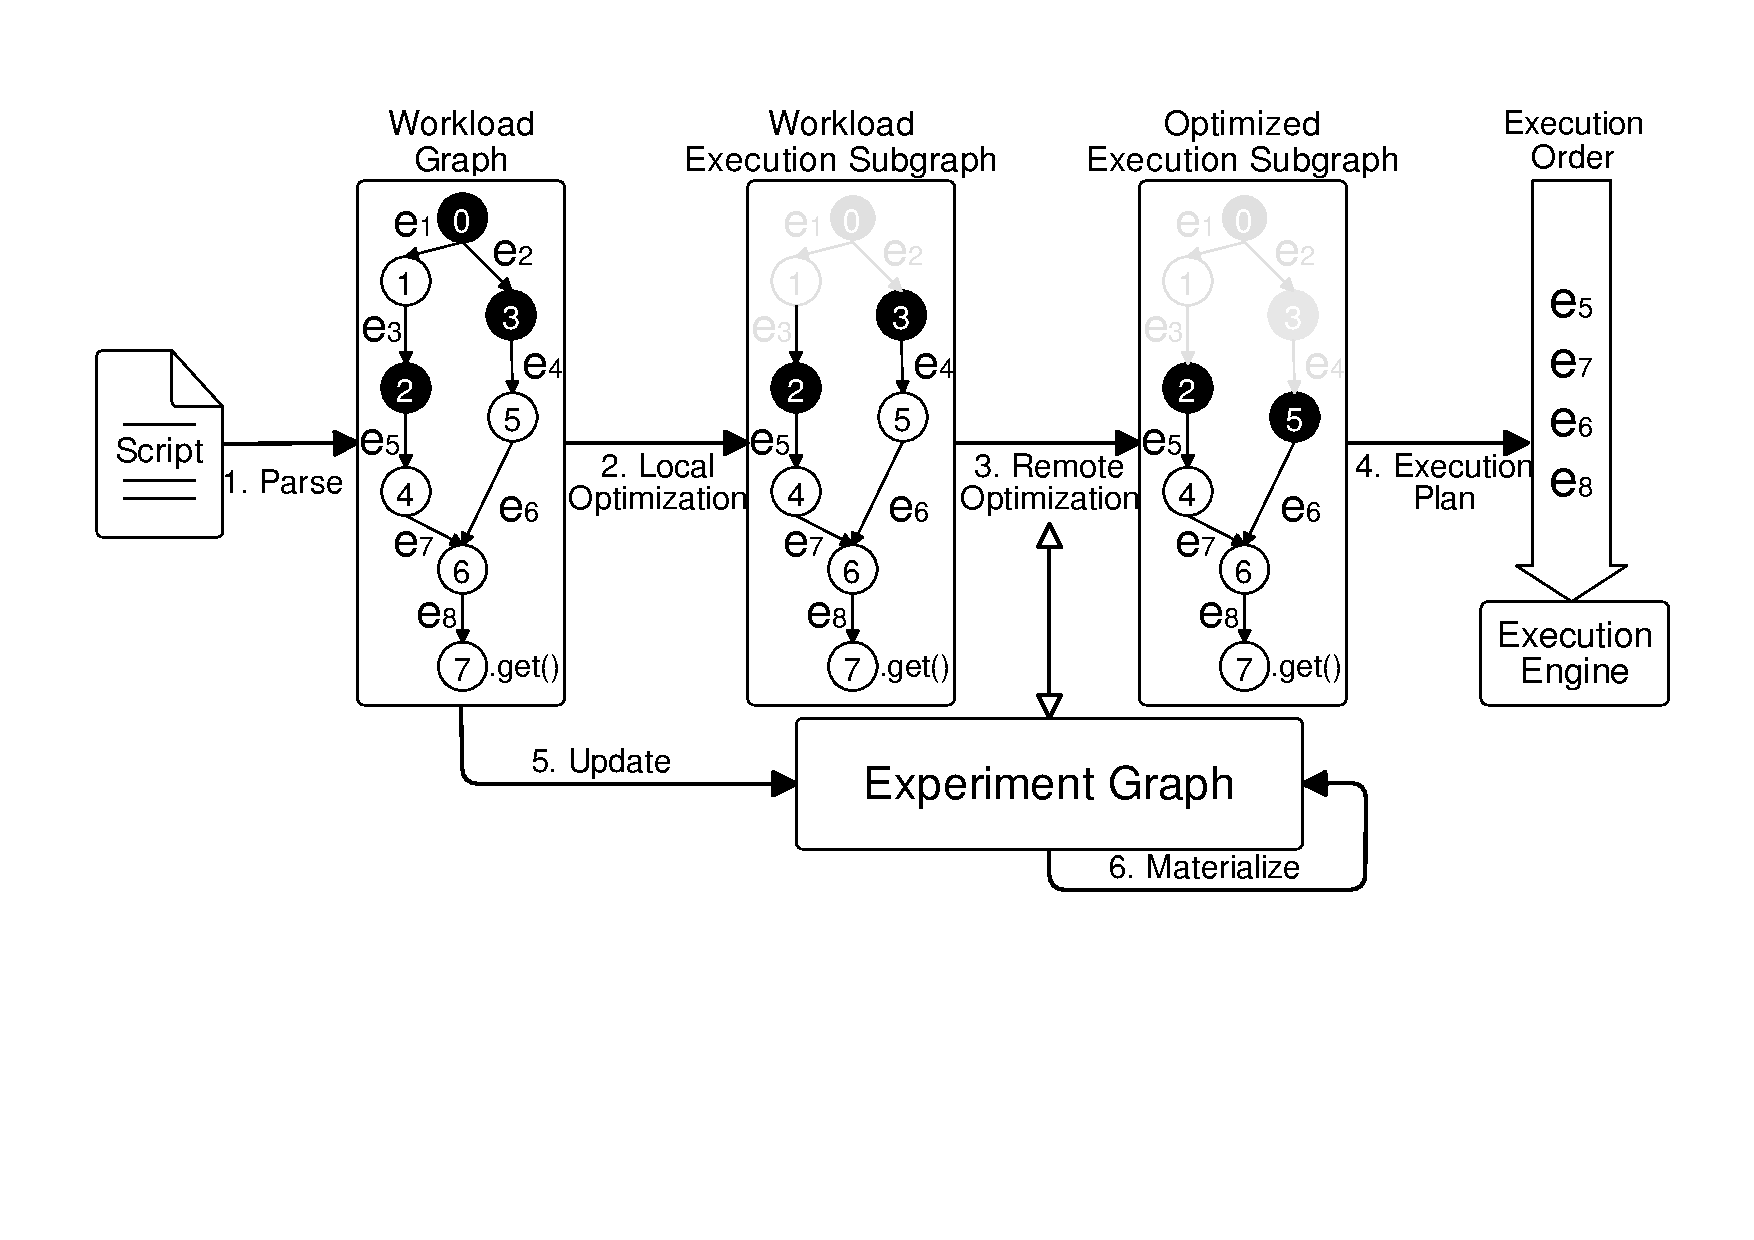
\includegraphics[width=0.7\columnwidth]{../images/system-workflow}
\caption{System overview of the collaborative workload optimizer}
\label{system-workflow}
\end{figure}

\subsection{Workload Optimizer for Kaggle Use Case}
\hl{In this section, we describe how our system can be integrated into Kaggle's collaborative data science platform to improve the execution of the kernels.
We select the competition \textit{Home Credit Default Risk}\footnote{https://www.kaggle.com/c/home-credit-default-risk/}.
The task of the competition is to train a classification model which predicts whether a client is able to repay their loans.
The task has 8 training datasets and 1 test datasets.
\todo[inline]{explain ROC}
The goal of the submitted solutions is to maximize the evaluation function, the area under the ROC curve between the predicted values and observed target values.
After a kernel is submitted, it goes through every step of the workload optimizer system in Figure \ref{system-workflow}.
For every competition, we maintain a separate experiment graph.
At the time of the first kernel submission, the experiment graph is empty, therefore, the workload optimizer system skips Step 3 of Figure \ref{system-workflow} and generates the execution plan directly from the workload execution subgraph.
If the experiment graph is not empty, the global optimizer tries to optimize the workload using the experiment graph.
For example, the most popular kernel\footnote{https://www.kaggle.com/willkoehrsen/start-here-a-gentle-introduction} in the competition has been copied by more than 5000 different users.
This indicates the kernel has been executed at least 5000 times, although it is very likely that many of the users run the script more than once.
Each execution of the kernel takes nearly 200 seconds.
In our experiments, we show that we are able to reduce the execution time to less than 10 seconds when the same kernel is executed more than once.}